\documentclass{article}
\usepackage[OT1]{fontenc}
\usepackage{microtype,graphicx,booktabs,amsmath,amssymb,array,xurl}
\usepackage[hypertexnames=false]{hyperref}
\usepackage{mlsys2025}
\makeatletter
\renewcommand{\Notice@String}{Scientific baseline v0.12.0. Author review draft; not submitted.}
\makeatother
\hypersetup{pdfauthor={Anonymous Authors},pdftitle={State and Cost Limits of Reference-Preserving Speculative Decoding},pdfsubject={Scientific baseline v0.12.0}}
\newcommand{\R}{R}
\newcommand{\M}{M}
\newcommand{\C}{C}
\mlsystitlerunning{State and Cost Limits of Reference-Preserving Speculation}
\begin{document}
\twocolumn[{
\mlsystitle{State and Cost Limits of Reference-Preserving Speculative Decoding}
\begin{mlsysauthorlist}\mlsysauthor{Anonymous Authors}{anon}\end{mlsysauthorlist}
\mlsysaffiliation{anon}{Anonymous Institution}
\mlsyscorrespondingauthor{Anonymous Author}{anon.email@domain.com}
\mlsyskeywords{speculative decoding, numerical state, execution paths, consumer systems}
\vskip 0.3in
\begin{abstract}
Matching a fixed decoder's output and accelerating it are separate requirements for speculative execution. We study their interaction in quantized consumer-system deployments, using natural retained-state crosses, complete-output qualification, and paid ordinary and matched-path baselines. On RTX, crossing historical state with the current verification path reveals both path effects and state--path interactions at selected boundaries. A local attention-layout constraint, applied to target prefill and continuation, preserves the measured reference on 24 previously unused project inputs. Its generation and resident-request speedups are 1.170$\times$ and 1.742$\times$ against the paid scalar reference; the corresponding gains against matched draft-free execution are 1.169$\times$ and 1.035$\times$. The distinction matters: the matched path already delivers 1.683$\times$ request speedup without speculation. Increasing draft length at fixed microbatch capacity preserves outputs on a separate panel but increases latency despite fewer target calls. On B570, a different phase-binding repair recovers finite reference endpoints while remaining slower than ordinary decoding. Historical M4 and 358H studies delimit additional performance opportunities. These results establish bounded state/path and cost counterexamples, plus a concrete positive RTX instance. They do not establish a universal repair, unique kernel cause, or architecture-independent determinism.
\end{abstract}
}]
\printAffiliationsAndNotice{}

\section{Introduction}
Speculative decoding replaces some sequential target-model work with drafting and parallel verification~\cite{leviathan2023}. Its mathematical output-distribution guarantee does not imply reproduction of a particular floating-point deployment's greedy token sequence. Prefill, continuation, verification, and cache reuse can select different numerical computations. Even when two executions have committed the same token prefix, their retained numerical states can differ. The resulting differences may influence later verification decisions.

Existing work addresses important parts of this problem. Batch-invariant inference fixes numerical reduction choices~\cite{thinkingmachines}; LLM-42 combines fixed-shape verification with consistent KV state~\cite{llm42}; Stage-Replay directly transplants KV caches~\cite{stagereplay}; and Vosti specifies and verifies determinism across engine and kernel behavior~\cite{vosti}. These precedents prevent us from claiming that state consistency, fixed verification, or selective numerical constraints are new principles. Our question is narrower: \emph{in a measured quantized deployment, which combinations of historical state and current execution preserve its reference, and does the resulting speculation still amortize verification?}

We answer through an empirical sequence rather than a general-purpose decoding algorithm. Native state crosses separate the retained numerical state from the next execution recipe. A finite constraint family then varies target/draft and prefill/continuation scope. Output qualification precedes speed claims, and two draft-free comparators distinguish the total deployment-path change from the increment obtained by speculation. Width and backend experiments expose where a qualified transformation fails to pay.

Three results form the contribution. First, natural state--current-path matrices on CUDA and Vulkan include current-path effects, interactions, state effects under duplicate current controls, and local null effects. Second, a query-local RTX implementation retains batched projections and feed-forward operations while reproducing finite scalar references; expanded-input measurements support positive generation performance against both ordinary and matched baselines. Third, jointly reporting reference and cost boundaries exposes two misleading proxies: fewer target caller invocations can accompany slower qualified decoding, and improvement over an old speculative implementation can coexist with a large regression against ordinary decoding.

The reusable contribution is the experimental separation of these quantities and its concrete counterexamples. The implementation recipes differ between GPUs. The strongest late evidence uses one model family; four platforms with measurements are not four replications of one causal mechanism. We retain these limits throughout, rather than pool unlike contracts into a universal speedup.

\section{Reference, State, and Cost Contracts}
\label{sec:contracts}
Fix model weights, tokenizer, prompt format, sampler, runtime, backend, and an output endpoint. Let $R(x)$ denote the paid ordinary reference for input $x$. Qualification checks submitted token IDs, length, terminal token when available, and stop reason. It is an output-reproduction requirement, not code correctness, equal logits, or a proof of distributional equivalence.

The RTX expansion compares the full saved response arrays through the runtime EOG or token cap. For B570, the registered endpoint is the prefix through the first runtime EOG or token 128. Extra raw suffix tokens can therefore coexist with qualified endpoints; their actual work remains included in the measured candidate cost. These contracts must not be interchanged.

At a natural boundary with committed prefix $p$, denote the retained state by $s$ and the current execution recipe by $e$. The observed decision is
\begin{equation}
 d = F(p,s,e).
\end{equation}
The state includes numerical KV contents and relevant runtime state, not merely token IDs. Crossing naturally reached states $s_0,s_1$ with recipes $e_0,e_1$ produces four observations. Differences between columns within a row demonstrate a current-recipe effect for that state. Differences between rows within a column demonstrate a donor-state effect. A recipe effect present under only one donor is a local interaction. These are observations at selected boundaries, not a unique-operation attribution or a global functional decomposition of $F$.

For timing, let $t_{i,b}$ and $t_{i,c}$ be each task's medians of absolute baseline and candidate costs over the campaign's repetitions. We report
\begin{equation}
 S_{b/c}=\exp\left(\frac{1}{n}\sum_{i=1}^{n}\log\frac{t_{i,b}}{t_{i,c}}\right).
\end{equation}
Values above one favor the candidate. Repetitions are not independent tasks. Intervals resample tasks after collapsing repetitions and describe the measured panel, rather than a model-family or hardware population.

Two comparators answer different questions. Ordinary $R$ measures the full improvement over the selected paid reference. Matched $M$ uses the candidate target path and prefill configuration without drafting, measuring speculation's increment on that path. Candidate $C$ combines that target path with native drafting. For the same tasks, timers, and aggregation,
\begin{equation}
 S_{R/C}=S_{R/M}S_{M/C}.
\label{eq:identity}
\end{equation}
This is an arithmetic identity, not a component-cost model. Differences in prefill or continuation cannot be converted into measured kernel fractions without profiling. Nor does a qualified $R$ establish the fastest possible ordinary decoder.

\section{Experimental Sequence and Evidence Strength}
The late RTX studies use an RTX 5070 Ti Laptop, Qwen3-8B/Qwen3-0.6B Q8\_0, the frozen non-flash CUDA graph, one service slot, greedy sampling with seed 123, context 4096, and 24 host threads. Local code is bound separately from upstream binaries and the public experiment-repository commits. New input eligibility is audited before reference generation. The accessible history leaves 24 eligible MBPP inputs for expansion; it does not leave the initially planned unused HumanEval panel. Thus input transfer means previously unused in this project, not absent from pretraining or a new model architecture.

The sequence has distinct evidence roles: four exposed native-state probes; a 16-mask exposed factorial; 19-task qualification and cost panels; the frozen 24-input expansion; width/length boundary tests; and a resident serial-request reset study. Earlier screening results motivated experiments but are not pooled with confirmation costs. Output traces used in causal discovery are not advertised as a holdout.

The RTX expansion has four conditions, 24 tasks, and four repetitions: 384 formal paid requests, plus 16 excluded warmups. Each condition has 96 qualified responses. References are stable across repetitions; output lengths range from 11 to 128, with 23 tasks ending at EOG and one at the cap. Formal timing disables diagnostic capture. Sessions use balanced condition-specific order; the comparison is a resident single-request campaign, not concurrent production throughput.

The final ordinary-reference analysis reconstructs costs from that existing campaign on CPU. It adds no model requests, forwards, warmups, or independent hardware replication. Original-host verification inspected the saved arrays, archive and timer bindings. The integration review independently recomputed the public 384-row cost export, 4,320 derived numeric table entries, all 12 comparison summaries, and their task-bootstrap intervals. This latter check does not independently reopen every private raw archive or authenticate omitted weights and runtime assets.

The B570 experiment uses its own Qwen3/Vulkan deployment and phase-binding recipe. Its endpoint and cost records are separately audited. Historical M4 and Core Ultra 358H data keep their own references, timers, and models. Source-specific denominators are retained; repetitions or repeated cap contexts never inflate the number of independent inputs.

\section{Natural State Crosses}
\label{sec:cross}
\subsection{RTX: path effects and local interactions}
Four previously exposed HumanEval probes use naturally reached donor states at equal committed prefixes. Across repetitions, 24 donors generate 48 state/current-path forks with 24 own-path shams. Auxiliary probe forwards are separately charged and are not speed measurements. Restoring and continuing an own-path state checks that the manipulation itself reproduces the native decision.

At HumanEval/15, the final verification/bonus decision changes with the current UB2 versus UB1 call under both donors. At HumanEval/25, only the combination of the N1 donor and current UB1 call changes the sampled decision. The latter is an interaction, not a state-only explanation. At the chosen boundaries of /18 and /31, neither intervention changes the discrete decision. A null at these boundaries does not prove trajectory-wide invariance.

The donors' prompt K/V tensors agree in all 12 compared pairs, while 70 of 72 generated-prefix tensor comparisons differ. First-layer logical K/V remain equal in the tested pairs. This narrows the descriptive state difference but does not identify attention as the unique cause. The /15 bonus-row observation also shows why the immediate scalar sample shape alone cannot describe the whole numerical history.

The expanded width study supplies another case. MBPP/229 at a natural 47-token prefix fails at wide UB6 verification. Real donor-state crosses under two current query layouts flip EOG argmax with the state; current layout changes continuous scores without independently flipping argmax in the measured cells. Four shams reproduce their own decisions. Two cap contexts are two observations of one task, not two independent counterexamples. This case connects a numerical-state boundary to a wider qualified-execution search without claiming a uniquely causal CUDA kernel.

\subsection{B570: a different recipe and the same questions}
On B570, six natural-state crosses with 12 own-path shams cover three tasks in repeated contexts. Byte-validated round trips and KV ownership checks support genuine donor-state manipulation. HumanEval/145 and /42 show local state--whole-recipe interactions. MBPP/72 shows a donor-state effect while its two current-recipe columns are identical controls. It cannot count as an independently varied current-path effect.

Table~\ref{tab:cross} shows representative raw argmax IDs, whose numeric magnitudes have no metric interpretation. The current B570 recipes change microbatch and output-reservation behavior together. The matrix therefore does not isolate one operator. Subsequent counterfactual complete continuations are not available for these cross cells; endpoint recovery is demonstrated separately by native full requests.

\begin{table}[t]
\centering\footnotesize\setlength{\tabcolsep}{3pt}
\caption{Representative B570 $2\times2$ argmax matrices. Rows are natural donor states; columns are the recorded current recipes. /72 has duplicate columns. Cases are local evidence, not prevalence estimates.}
\label{tab:cross}
\begin{tabular}{lcc}\toprule
Task & Donor 0: $(e_0,e_1)$ & Donor 1: $(e_0,e_1)$\\\midrule
HumanEval/145 & $(71465,279)$ & $(279,279)$\\
HumanEval/42 & $(432,1817)$ & $(1817,1817)$\\
MBPP/72 & $(320,320)$ & $(308,308)$\\\bottomrule
\end{tabular}
\end{table}

Together the two GPUs support the portability of the \emph{experimental question}: equal prefixes do not remove the need to control retained state and the current recipe. They do not demonstrate that one constraint, matrix pattern, or parameter choice transfers unchanged between CUDA and Vulkan.

\section{A Finite RTX Repair with Two Baselines}
\subsection{Local layout and scope}
The RTX implementation changes the query layout of the Qwen3 non-flash attention subgraph using existing ggml views and CUDA operations. Query columns are represented in the batch dimension so that attention follows the selected scalar-query structure; projection and feed-forward operations retain their batched execution. This is a local graph transformation, not a new CUDA kernel or architecture-independent arithmetic proof.

Four switches apply the constraint to target prefill, target continuation, draft prefill and draft continuation, encoded by bits 1, 2, 4 and 8. The exposed factorial contains 16 masks, four probes and two repetitions, totaling 128 complete requests. Masks 3, 7, 11 and 15 pass every registered reference endpoint. Mask 3 is inclusion-minimal within this finite family. /15 and /31 pass all masks; /25 needs either target phase; /18 needs both. Draft constraints are unnecessary for qualification on this panel. That observation does not establish global minimality or automatic constraint discovery.

Mask 3 is chosen by output qualification, not observed speed. On 19 exposed tasks, the subsequent six-repetition panel yields 1.27808$\times$ generation and 1.11298$\times$ resident-request speed against matched target-only execution. Removing draft constraints relative to mask 15 adds only 1.00357$\times$ generation and 1.02569$\times$ request speed. The extra generation benefit misses the predeclared 1.03$\times$ gate, and its descriptive interval crosses one. We retain the positive matched-path result without claiming that minimal scope itself provides an additional robust decode optimization.

\subsection{Expanded input measurements}
The frozen mask-3, $k=3$, UB4 recipe qualifies all 96 candidate responses on the 24-input MBPP expansion. The all-scope and matched-target conditions also qualify. Table~\ref{tab:cost} reports the final paid-reference reconstruction from the same campaign. The ordinary condition is mask 0, UB1, draft-free execution in the qualified frontend. It is a real measured scalar reference, not an unmeasured optimum over all possible decoding implementations.

\begin{table*}[t]
\centering\small\setlength{\tabcolsep}{3pt}
\caption{RTX expansion: 24 tasks, four repetitions per condition. Baseline/candidate geometric mean of task-median absolute times; above one favors the candidate. Brackets are descriptive task-bootstrap 95\% intervals. Ordinary $R$ and matched $M$ are both draft-free.}
\label{tab:cost}
\begin{tabular}{lcccc}\toprule
Comparison & Generation speed & Resident-request speed & Generation faster & Request faster\\\midrule
$R/C$: ordinary / mask-3 speculation & $1.17012\ [1.11701,1.21768]$ & $1.74157\ [1.65461,1.82708]$ & 22/24 & 24/24\\
$M/C$: matched / mask-3 speculation & $1.16924\ [1.11711,1.21715]$ & $1.03507\ [1.00455,1.06348]$ & 22/24 & 17/24\\
$R/M$: ordinary / matched draft-free & $1.00076\ [0.99529,1.00775]$ & $1.68256\ [1.58980,1.76633]$ & 11/24 & 24/24\\\bottomrule
\end{tabular}
\end{table*}

Both generation comparators support a finite positive result. The request result requires more care. Matched draft-free execution already achieves 1.68256$\times$ against ordinary $R$, whereas adding speculation on that path contributes 1.03507$\times$. The 1.74157$\times$ total gain must therefore not be described as entirely caused by speculation. Equation~\ref{eq:identity} holds for all 48 task-level generation/request identities and both aggregate identities. It apportions comparisons, not measured implementation components.

The matched-request result is modest and uneven: seven tasks are slower, and repetition 2 has aggregate speed 0.94022$\times$. The four ordinary-reference request repetitions are approximately 1.726, 1.736, 1.727 and 1.737$\times$. Within-task medians and balanced session order expose variability but cannot eliminate thermal drift or condition-specific session confounding on a laptop. Intervals do not turn this campaign into independent multi-day replication.

The generation timer is the original server \texttt{predicted\_ms} field. It excludes prompt processing, the first sample and some final bookkeeping. Resident-request time is host HTTP response wall time, including prefill, generation, transport and client parsing. It excludes loading, warmup and shutdown and may exclude asynchronous post-response cleanup. The $R$ versus $M$ comparison changes prefill microbatch/attention behavior as well as continuation capacity. No per-component timing establishes where its large request gain is spent. The target-state transplant branch is disabled in this campaign; code availability is not evidence that transfer cost was paid here.

\begin{figure}[t]
\centering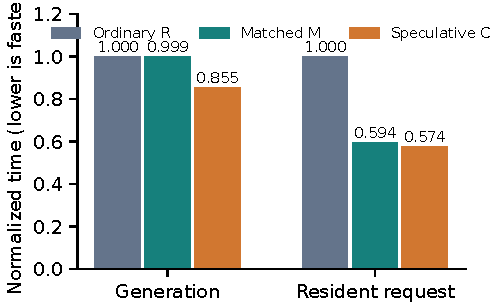
\includegraphics[width=\linewidth]{figures/reference_cost.pdf}
\caption{RTX expansion costs normalized task-by-task to ordinary $R$, then geometrically averaged. Matched draft-free execution already reduces request cost substantially. Bars are aggregate ratios, not additive component fractions.}
\label{fig:reference}
\end{figure}

\section{Qualification and Amortization Boundaries}
Table~\ref{tab:boundary} summarizes the distinct outcomes. Passing the output gate does not imply passing the cost gate, and a failed output gate disqualifies a speed claim even if the recorded run is fast. The rows come from separate registered panels; they are not a pooled benchmark.
\begin{table}[t]
\centering\footnotesize\setlength{\tabcolsep}{3pt}
\caption{Observed qualification/cost combinations. Gen./req. speeds are against the named draft-free baseline; -- means no qualified speed claim.}
\label{tab:boundary}
\begin{tabular}{lccc}\toprule
Recipe & Qualified panel & Baseline & Gen./req.\\\midrule
RTX $k=3$, UB4 & 24 tasks & Matched & 1.169/1.035\\
RTX $k=7$, UB4 & 28 tasks & Matched & 0.997/0.950\\
RTX $k=7$, UB8 & Fails /229 & -- & --\\
B570 $k=2$ repair & 15 tasks & Ordinary & 0.283/0.201\\\bottomrule
\end{tabular}\end{table}
\subsection{Changing geometry can break the repair}
The expansion into draft length and microbatch capacity keeps failed cases. At paired $(k,\mathrm{UB})=(1,2)$ and $(3,4)$, the tested width/length panel qualifies. MBPP/229 fails at $(5,6)$ and $(7,8)$ under all measured cap contexts and repetitions, even though its wide ordinary and matched paths pass. The old HumanEval/18 probe also supplies an outside-panel failure at wider target-only capacity. Increasing the output cap does not certify every trajectory to that length: some responses finish much earlier, with observed maximum length 261 rather than a full 512-token stress trajectory.

A separate experiment holds UB4 fixed and tests $k=3,5,7$. All 28 exposed qualification tasks pass in two repetitions. The widest $k=7$ recipe is selected by qualification only, then measured in independent capture-off cost sessions. Against $k=3$, it obtains 0.82944$\times$ generation and 0.88987$\times$ request speed: qualified outputs, slower execution. Against matched target-only, $k=7$ reaches 0.99740$\times$ generation and 0.95035$\times$ request speed; the $k=3$ anchor reaches 1.20250$\times$ and 1.06797$\times$. Larger $k$ is neither a monotone correctness repair nor a monotone performance improvement in these contracts.

Diagnostic sessions, including warmup, record target caller calls falling from 305 to 199 while observed micrographs rise from 305 to 397. Separate formal work records show drafted tokens increasing from 3528 to 5392 and accepted tokens from 2772 to 3192. These are different sessions and must not be divided into one fabricated per-call measure. Micrograph observations are not CUDA kernel launches. The counts reveal why caller reduction is an inadequate performance proxy; they do not uniquely prove which component caused the slowdown. This limitation is consistent with prior work on verification cost~\cite{illusion}, while the fixed-capacity, reference-qualified counterexample adds a concrete numerical-contract boundary.

The resident serial-request study verifies reset behavior and positive finite costs on its own panel, approximately 1.181$\times$ generation and 1.039$\times$ request against its matched comparator. It is not a throughput or concurrency benchmark and is not pooled with the expansion.

\subsection{B570: repair without deployment gain}
The B570 frontend combines ordinary-reference prompt construction, in-place prefill-to-continuation phase binding from UB128 to UB1, and the existing $k=2$, draft-UB1 speculative loop. It qualifies 12 development requests, 112 requests over 56 exposed tasks, and all 30 candidate requests over 15 inputs unused in the accessible project. Qualification is the cap-128 endpoint contract from Section~\ref{sec:contracts}. The 30 candidate responses include extra raw suffix differences; endpoint equality cannot be rewritten as raw-array equality.

The formal E matrix is 119/120 complete because one old-N1 request lacks a payload. Ordinary $R$, matched target-only, and the candidate each have all 30 paid observations, so their 15 task-median pairs remain complete. Candidate speed is 0.28259$\times$ generation and 0.20129$\times$ request against ordinary $R$, slower in every paired round. Against matched target-only it is 0.28576$\times$ and 0.20570$\times$. Matched target-only itself is near the ordinary reference: 0.98889$\times$ and 0.97854$\times$. Thus the entire candidate regression cannot be attributed to a target consistency constraint alone.

Against 14 complete old-N1 task pairs, the candidate improves generation/request by 3.99309$\times$/2.63394$\times$, with a single request-round reversal at MBPP/245. This old-implementation improvement does not establish a deployable gain. Draft, accepted, caller and extra-suffix work are recorded, but no independent component profile identifies a unique remaining bottleneck. Further GPU investment in this exact route is not supported by these measurements.

\subsection{Historical opportunities on M4 and 358H}
Historical M4 measurements provide a positive counterweight to the negative consumer results. A prospective 60-task panel, 30 HumanEval plus 30 SpecBench inputs, has three conditions and three repetitions: 540 requests. Fixed Always speculation and Guard each qualify 180/180 responses under that study's contract. Their post-prefill speedups against target-only are 1.34689$\times$ and 1.31139$\times$. Guard is 2.71\% slower than Always in geometric task latency. This does not mean adaptive speculation is universally ineffective; it means this guard lacks a measured advantage on this prospective panel.

A whole-request offline oracle choosing between target-only and Always by each observed task's medians improves on Always by only about 0.0692\% in geometric mean. It is a panel-specific choice oracle, not an upper bound for intra-request policies or other implementations. On Core Ultra 358H, CPU and NPU drafting reproduce the reference on their 90-request panels but yield 0.73392$\times$ and 0.35166$\times$ speed. Conditional removal of measured overhead leaves the available ceilings below parity. Full-prefix NPU replay and the historical target path are properties of that implementation, not impossibility results for heterogeneous decoding.

These older studies constrain the practical interpretation of the late repair work. They do not replicate the RTX/Vulkan state-cross mechanism and do not supply additional independent architecture transfer for the local constraint.

\section{Related Work and Contribution Overlap}
Speculative decoding's sampling guarantee~\cite{leviathan2023}, heterogeneous execution~\cite{dovetail,duodecoding}, and adaptive depth control~\cite{turbospec,banditspec} are established directions. Consumer-hardware numerical deviations and serialization costs have also been studied~\cite{lossless}. We therefore present neither heterogeneous drafting nor consumer slowdown as an original general concept.

LLM-42 fixes verifier shapes, maintains consistent KV state and supports selective deterministic requests~\cite{llm42}. Its principles overlap our decision to preserve a constrained target path while allowing draft freedom. Our empirical scope mask is not a first selective-determinism theorem. Vosti supplies a broader system specification and formal engine/kernel argument~\cite{vosti}; our finite token/endpoint qualification is a weaker guarantee. MarginGate uses calibrated sparse verification~\cite{margingate}; we do not execute its method and cannot claim superiority or refutation.

Stage-Replay uses fixed prefixes, construction controls and bidirectional cache transplantation~\cite{stagereplay}. We share its premise that numerical state matters. Our additional measured factor is the current native execution recipe crossed with natural retained state, linked to a finite target-layout repair and a separately measured performance boundary. Prior cache-transplant evidence prevents a priority claim for state intervention itself.

\emph{Performance or Illusion?} analyzes target verification, acceptance variation and performance bounds on a production inference engine~\cite{illusion}. Fewer caller calls failing to produce proportional speedup is not a new general observation. Our increment is the coupled correctness/cost experiment at fixed microbatch capacity, with both ordinary and matched-path comparisons. There is no direct comparative implementation against LLM-42, Vosti or MarginGate on a shared contract; that remains a substantial method-paper limitation.

The project name also coincides with an ACL paper on contextual heterogeneity~\cite{aclheterospec}. That paper studies uncertainty-based verification allocation. We use a distinct descriptive manuscript title and cite it to avoid implying identity or priority based on the name.

\section{Limits and Implications}
The strongest positive result is an input-expanded RTX instance. It does not establish cross-family, stochastic-sampling, multi-slot, long-context, or flash-attention generality. The late causal and repair work predominantly uses Qwen3. B570 transfers the diagnosis questions and yields a different finite repair, but fails the ordinary-reference cost gate. M4 and 358H contribute historical cost limits, not equivalent causal matrices.

State crosses are outcome-informed, selected-boundary interventions with finite shams. They support local counterexamples and interactions, not prevalence or unique operator causes. Scope minimality holds only in the 16-switch family. Matching observed tokens can mask differing logits or retained state, and endpoint contracts can mask raw suffix differences. Conversely, a failed reference-preservation gate is not automatically a functional-answer failure.

The RTX ordinary reference is paid and qualified, yet not proven to be the fastest ordinary decoder. The 1.683$\times$ matched-path request advantage and 1.035$\times$ speculation increment make this distinction operationally important. Independent profiling and broader method comparisons would be needed for a universal performance account. Our task bootstrap is descriptive; it does not remove session confounding or support calibrated acceptance probabilities.

The engineering implication is a three-step decision: separate retained state from current execution when diagnosing deviations; qualify complete registered outputs before comparing costs; and require gains against both the selected ordinary reference and a matched draft-free path. Each step removes a specific ambiguity. This procedure is useful beyond the measured patch, but the current evidence does not establish an automatic, architecture-independent repair system.

\section{Conclusion}
Reference-preserving speculation has coupled numerical and cost boundaries. Natural state/current-recipe crosses reveal local effects that equal token prefixes alone cannot explain. A finite RTX target-layout constraint achieves positive generation performance against paid ordinary and matched comparators, while most of its ordinary-reference request improvement is already present without speculation. Fixed-capacity wider drafting and the B570 repair show that qualified execution can still lose its cost advantage. These results support a bounded empirical contribution and a concrete positive instance; the path to a general method requires evidence beyond the current family and implementation.

\label{maintextend}
\clearpage
\bibliographystyle{mlsys2025}\bibliography{references}
\end{document}
